\RequirePackage[]{paralist}
\documentclass[final]{beamer} % beamer 3.10: do NOT use option hyperref={pdfpagelabels=false} !
%
% IBS 2016 conference - POSTER
%
%                 Gundelfingen, 24.06.2019, Germany
%
%\documentclass[final,hyperref={pdfpagelabels=false}]{beamer} % beamer 3.07: get rid of beamer warnings
\mode<presentation> {  %% check http://www-i6.informatik.rwth-aachen.de/~dreuw/latexbeamerposter.php for examples
  \usetheme{Berlin}    %% you should define your own theme e.g. for big headlines using your own logos 
}
\mode<presentation>{\usetheme{I6pd2}}

\usepackage[english]{babel}
\usepackage[latin1]{inputenc}
\usepackage{amsmath, amsthm, amssymb, latexsym, upgreek, amsbsy, mathrsfs}
\usepackage{dcolumn}
\usepackage{multirow}
\usepackage{hhline}
\usepackage{booktabs}
\usepackage{caption}

\usepackage[absolute,overlay]{textpos}
\usepackage{graphicx}
\usefonttheme[onlymath]{serif}
\definecolor{orange}{RGB}{255,127,0}
\definecolor{yellowish}{RGB}{255,255,153}

\newcommand{\BM}[1]{\ensuremath{\mbox{\boldmath${#1}$}}}
\newcommand{\exedout}{%
  \rule{0.8\textwidth}{0.5\textwidth}%
}
\newcommand{\BraKet}[2]{\ensuremath{\bigl\langle {#1} \bigl\lvert {#2} \bigr\rangle}}
\newcommand{\tBraKet}[3]{\ensuremath{\bigl\langle {#1} \bigl\lvert {#2} \bigl\lvert {#3} \bigr\rangle}}

% ====================================================================================
\graphicspath{{figures/}}


\usepackage[orientation=portrait,scale=1.4,debug]{beamerposter}  
%
\title{\huge Fast Evaluation of Intermolecular Charge Transfer Energy: 
New Approach Based on One-Electron Effective Potentials
}
\author{\underline{Bartosz B{\l}asiak}, Joanna D. Bednarska, Marta Cho{\l}uj, Wojciech Bartkowiak}
\institute{
Department of Physical and Quantum Chemistry, Wroc{\l}aw University of Technology, Wroc{\l}aw 50-370, Poland}
\date[July. 4th, 2019]{July. 4th, 2019}

\setlength{\paperwidth}{84.0cm}
\setlength{\paperheight}{118.0cm}

% ==========================================================================================================================
\begin{document}

\begin{frame}{OEP-Based Charge Transfer (CT) Interaction Energy}

\begin{textblock*}{440mm}(10mm,135mm)
\begin{block}{Ab Initio Charge Transfer Energy in Fragment-Based Modelling}
 \begin{itemize}
   \item CT energy is an {\color{green} important} stabilizing contribution to the total interaction energy [1]
   \item It is {\color{red} very costly} to compute and generally not directly included in most force fields
   \item {\color{green} EFP2 model} implements efficient CT energy estomator [2,3]
   \item However, EFP2 CT energy is {\color{red} 30-40 times slower} then evaluating other components [3]
   \item In effect, this CT term is usually {\color{red} not included} in condensed matter modelling [4]
 \end{itemize}
\end{block}
\end{textblock*}

\begin{textblock*}{250mm}(10mm,253mm)
\begin{block}{Our Approach}
 \begin{itemize}
   \item Consider Murrell et al.'s perturbation theory [5]
   \item Apply OEP method to eliminate ERI's
   \item Adapt the CT term to the EFP2 method [2,3]
 \end{itemize}
\end{block}
\end{textblock*}

\begin{textblock*}{180mm}(270mm,253mm)
\begin{block}{CT energy by Murrell et al. [5]}
  \vskip-2ex
  \begin{equation*}
    \Delta E_{\rm CT}^{A\rightarrow B} = 2\sum_{i\in A}^{\rm Occ} \sum_{n\in B}^{\rm Vir}
     \frac{\vert V_{in}^{A\rightarrow B} \vert^2 }{\varepsilon_i - \varepsilon_n}
  \end{equation*}
  \vskip0.4ex
\end{block}
\end{textblock*}

\begin{textblock*}{367mm}(463mm,137mm)
\begin{exampleblock}{One-Electron Effective Potential (OEP) Operators}
OEP's can be introduced to eliminate electron repulsion integrals from parent theories:
\begin{equation*}
 \sum_t \sum_{ij} \sum_{kl\in A} \mathscr{F}_t 
 \left[ 
  \left< ij \vert k^A l^A \right>
 \right] 
  = \left<  
      i \vert \hat{v}^A_{\rm eff} \vert j
    \right>
\end{equation*}
\end{exampleblock}
\end{textblock*}

\begin{textblock*}{367mm}(463mm,233mm)
\begin{exampleblock}{Types of matrix elements of OEP operators}
\vskip0.1ex
\begin{table}[b]
\begin{tabular}{lcccc}
Matrix element      &&            `Overlap-like'                &&            `Coulomb-like'               \\ 
                    && $\tBraKet{i}{\hat{v}_{\rm eff}^{A}}{j} $ && $\tBraKet{j}{\hat{v}_{\rm eff}^{A}}{l}$ \\ 
	\cline{1-5}
Partitioning scheme &&            $i\in A, j\in B$              &&               $j,l\in B$                \\
Associated ERI's    &&            $\BraKet{AA}{AB}$             &&               $\BraKet{AA}{BB}$         \\
Handling            && Density Fitting                          && Distributed Multipoles                  \\
\end{tabular}
%
\end{table}
\vskip-0.1ex
\end{exampleblock}
\end{textblock*}

% - Graph 1
\begin{textblock*}{340mm}(10mm,807mm)
\begin{figure}
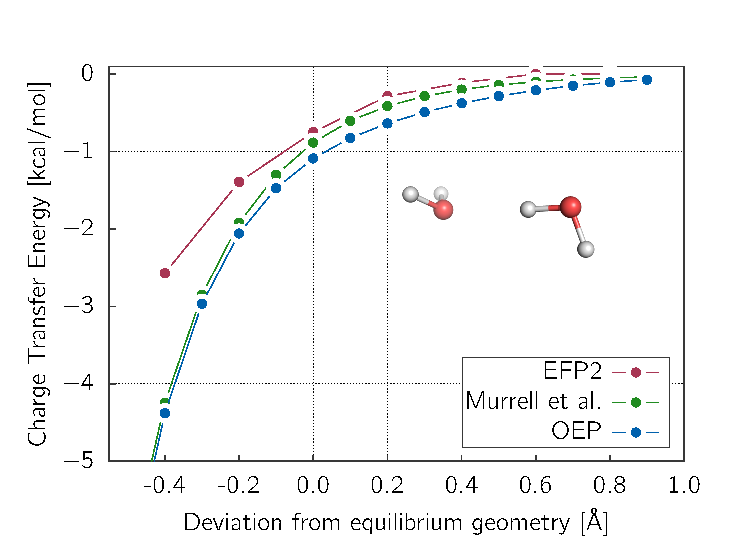
\includegraphics[width=1.0\textwidth]{fig-1-s.eps}
%\caption{\bf OEP-based model reproduces CT energies of the parent Murrell et al.'s [3] model.}
\end{figure}
\end{textblock*}

% - Arrow
\begin{textblock*}{60mm}(220mm,903mm)
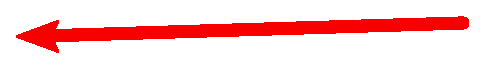
\includegraphics[scale=0.37]{arrow.eps}
\end{textblock*}

% - Graph 2
\begin{textblock*}{340mm}(290mm,820mm)
\begin{figure}
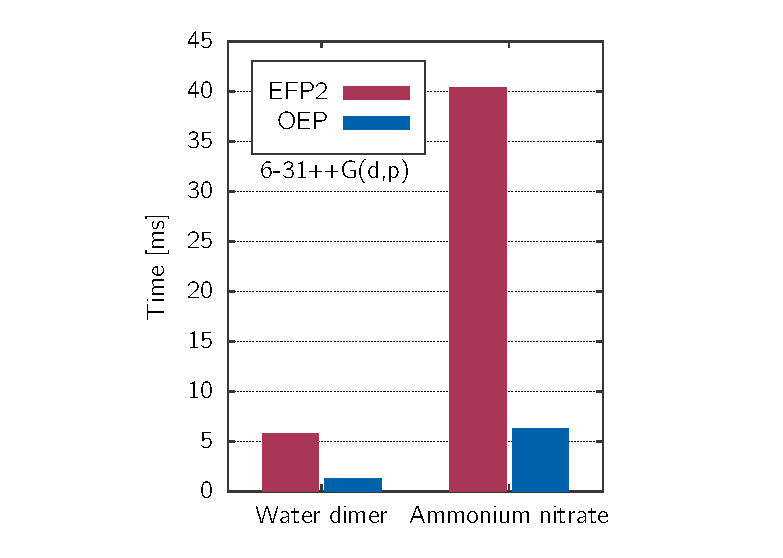
\includegraphics[width=1.0\textwidth]{fig-2.eps}
%\caption{\bf OEP-based model reproduces CT energies of the parent Murrell et al.'s [3] model.}
\end{figure}
\end{textblock*}


% - Scheme 
\begin{textblock*}{820mm}(10mm,341mm)
\begin{exampleblock}{Coupling Constant $\boldsymbol{ V_{in}^{A\rightarrow B} } $}
\begin{figure}
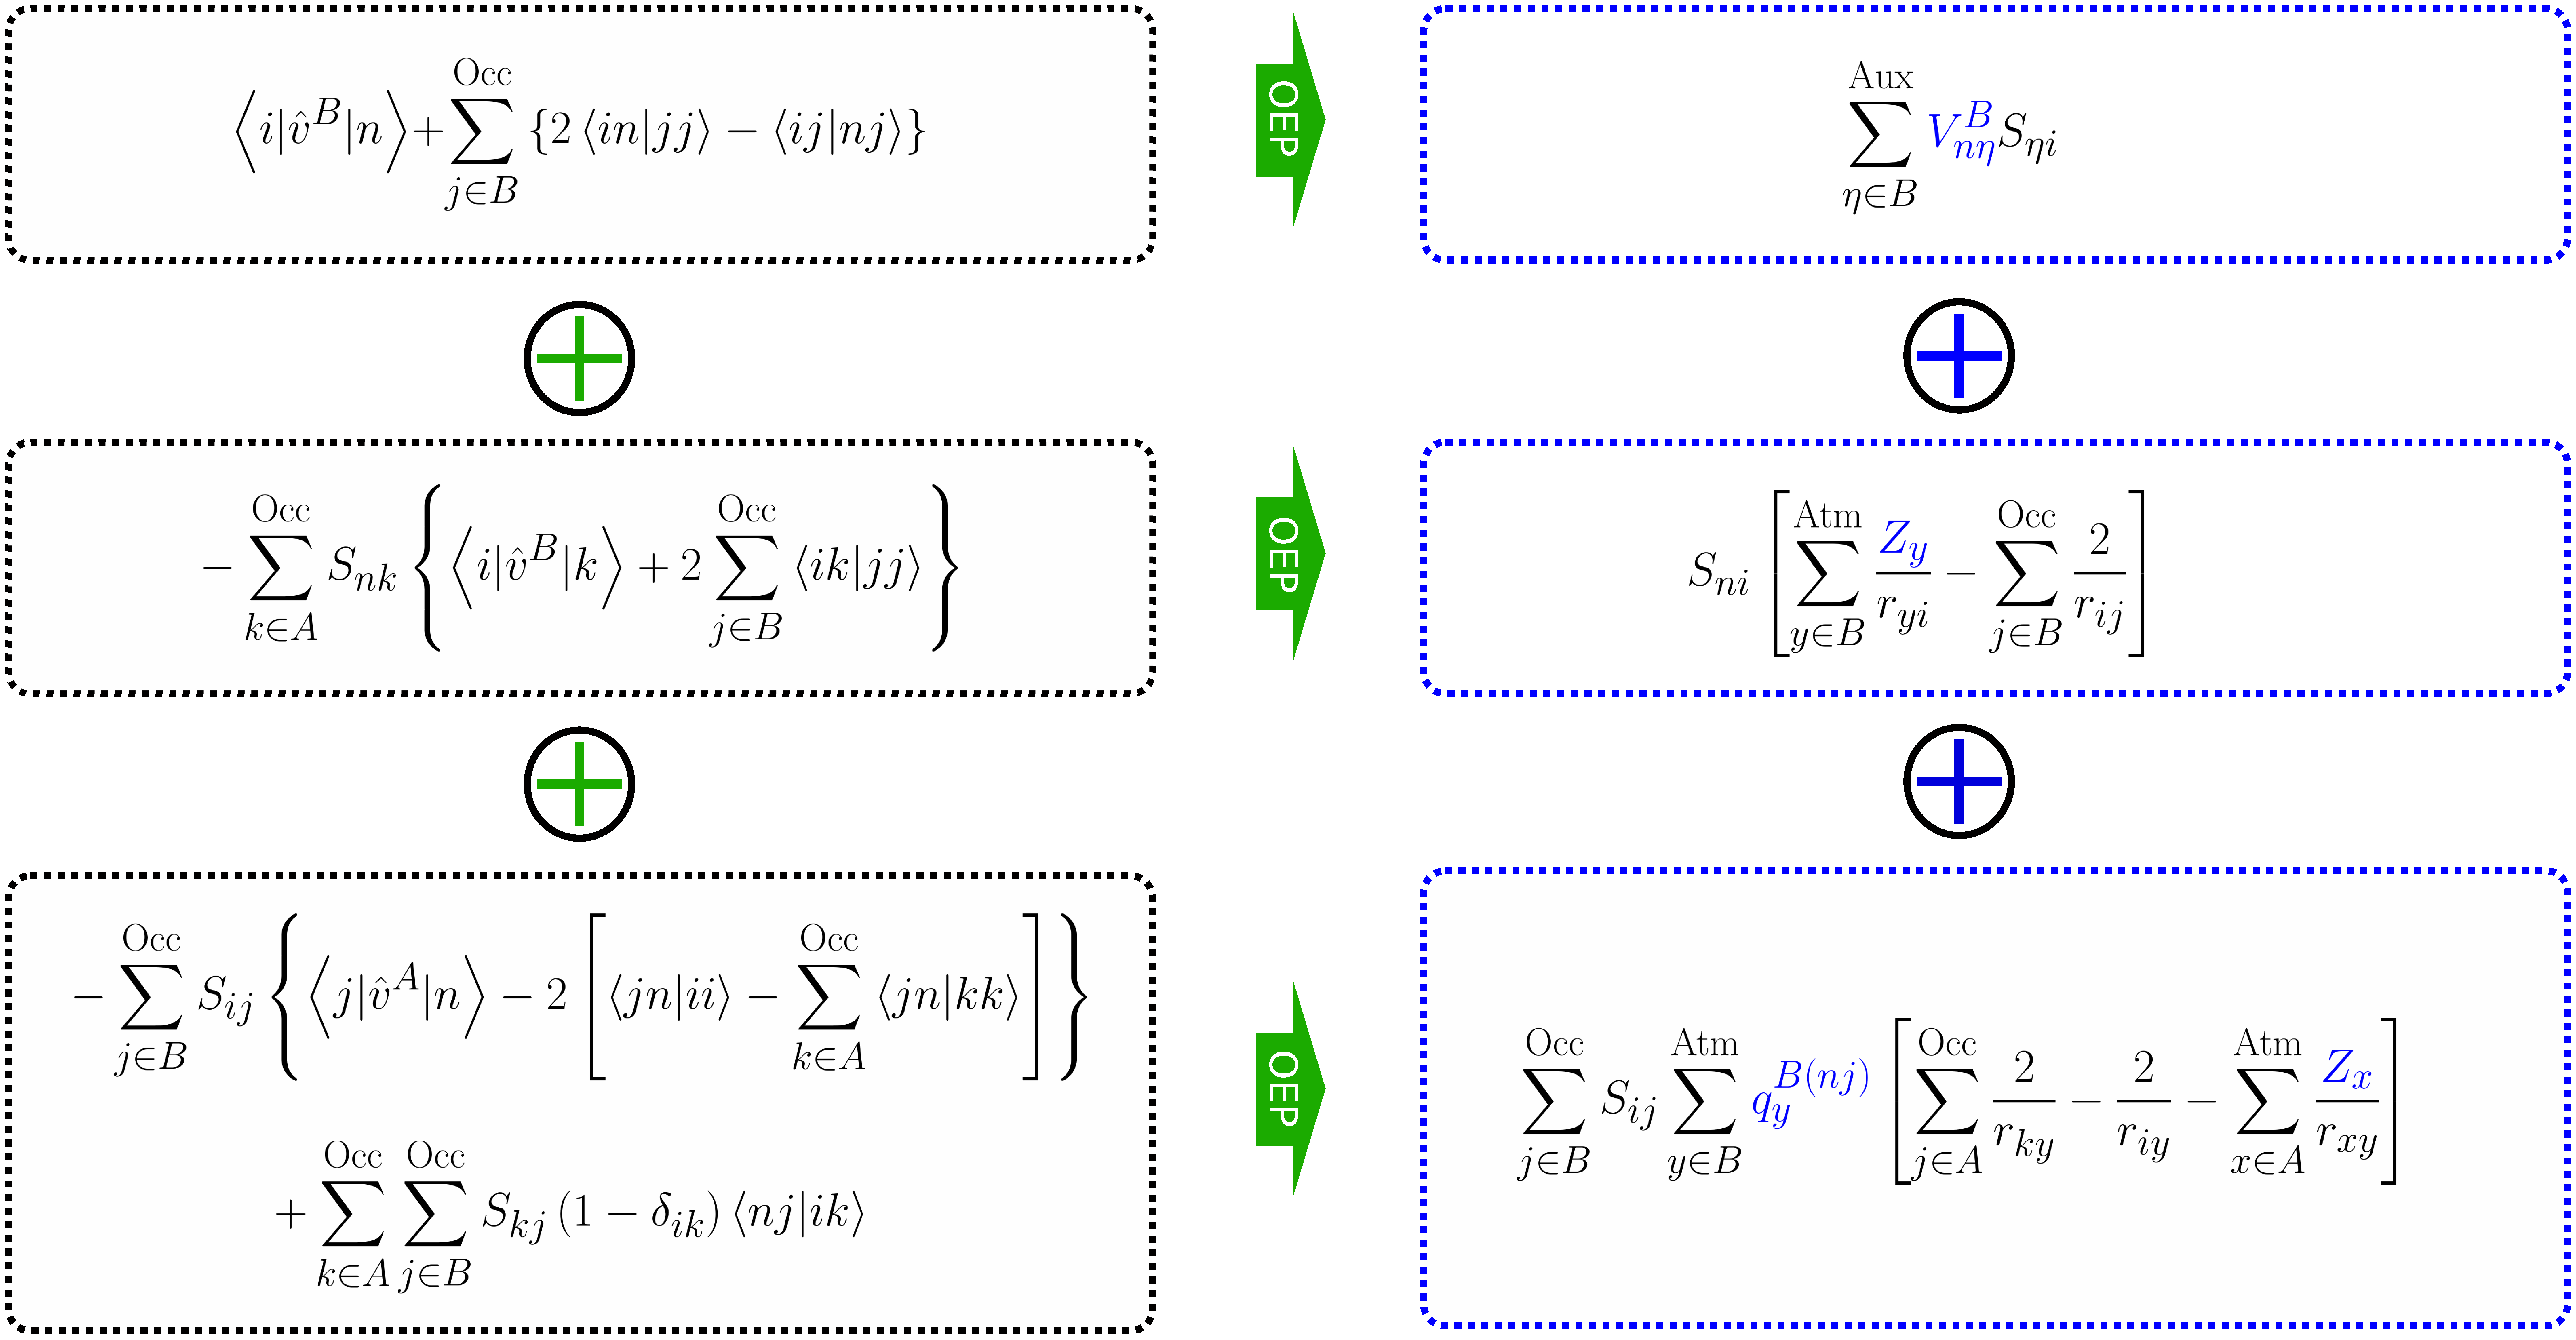
\includegraphics[width=1.0\textwidth]{scheme.eps}
\caption{\bf Application of the OEP technique to significantly simplify original theory of Murrell et al.[5] EFP parameters
are shown in blue.}
\end{figure}
\end{exampleblock}
\end{textblock*}

% ----- RULE DIVIDING THEORY AND RESULTS
\begin{textblock*}{820mm}(6mm,820mm)
\noindent\rule{83cm}{5.4pt}
\end{textblock*}

\begin{textblock*}{257mm}(573mm,824mm)
\begin{block}{Summary and Outlook}
 \begin{itemize}
   \item OEP-based model reproduces CT energies of the parent Murrell et al.'s [5] model
   \item OEP-based model is 4-7 times faster than EFP2
   \item Further optimization is possible: using QUAMBO orbitals [4]
   \item OEP's can be applied to other problems as well
 \end{itemize}
\end{block}
\end{textblock*}

\begin{textblock*}{257mm}(573mm,970mm)
%\begin{exampleblock}{\color{blue} References}
    References: %\\
    \begin{small}
%[1] Gordon, M. S.; Fedorov. D. G.; Pruitt, S. R.; Slipchenko L. V.; \emph{Chem. Rev.} {\bf 2012}, 112, 632
[1] Gordon, M. S. et al.; \emph{Chem. Rev.} {\bf 2012}, 112, 632 
[2] Li, H.; Gordon, M. S.; \emph{J. Chem. Phys.} {\bf 2006}, 124, 214108
[3] Xu, P.; Gordon, M. S.; \emph{J. Chem. Phys.} {\bf 2013}, 139, 194104
[4] Kaliman, I. A.; Slipchenko, L. V.; \emph{J. Comput. Chem.} {\bf 2015}, 36, 129
[5] Murrell, J. N.; Randic, M.; Williams O. R.; \emph{Proc. Roy. Soc. A} {\bf 1965}, 284, 566
    \end{small}         
%\end{exampleblock}
\end{textblock*}
\begin{textblock*}{257mm}(573mm,964mm)
\noindent\rule{83cm}{5.4pt}
\end{textblock*}




% ----- RULE DIVIDING RESULTS AND ACKNOWLEDGEMENTS
\begin{textblock*}{820mm}(6mm,1070mm)
\noindent\rule{83cm}{5.4pt}
\end{textblock*}


%
%
%% ----------------------- SUMMARY
%%
%
% --------------------- ACKNOWLEDGEMENTS
\begin{textblock*}{820mm}(10mm,1070mm)
\begin{block}{Acknowledgements}
 This project is carried out under POLONEZ programme which has received funding from the European Union's
 Horizon~2020 research and innovation programme under the Marie Sk{\l}odowska-Curie grant agreement 
 No.~665778. This project is funded by National Science Centre, Poland 
 (grant~no. 2016/23/P/ST4/01720) within the POLONEZ 3 fellowship.
 We thank
 Wroc{\l}aw Centre for Networking and Supercomputing (WCSS) for
 providing high quality computational resources.
\end{block}
\end{textblock*}


\end{frame}
\end{document}
